\documentclass[a4paper,12pt,twoside]{scrreprt}
% Autor der Vorlage: Klaus Rheinberger, FH Vorarlberg
% 2017-02-20

%% Hilfe: z.B.
% empfohlener Einstieg: http://latex.tugraz.at/
% https://de.wikibooks.org/wiki/LaTeX-Kompendium:_Schnellkurs:_Erste_Schritte
% https://de.wikibooks.org/wiki/LaTeX-Kompendium:_Schnellkurs
% https://de.wikibooks.org/wiki/LaTeX-Kompendium

%% Pakete:
% Der Befehl \usepackage[latin9]{inputenc} ermöglicht die direkte Angabe von Umlauten. Übrigens lässt sich so auch das Euro-Zeichen direkt eingeben. Auf Betriebssystemen, wie zum Beispiel allen neueren Linux-Distributionen, verwendet man statt \usepackage[latin9]{inputenc} besser \usepackage[utf8]{inputenc}, auf Applesystemen verwendet man \usepackage[macce]{inputenc} (oder das für ältere Modelle gültige \usepackage[applemac]{inputenc}).
\usepackage[utf8]{inputenc}
\usepackage[T1]{fontenc}    % Silbentrennung bei Sonderzeichen
\usepackage{graphicx}	    % Bilder einbinden
\usepackage[english]{babel} % Deutsche Sprachanpassungen
\usepackage{csquotes}	    % When using babel or polyglossia with biblatex, loading csquotes is recommended to ensure that quoted texts are typeset according to the rules of your main language.
\usepackage{acronym}  % für optionales Abkürzungsverzeichnis
\usepackage{eurosym}  % z. B. \EUR{12345,68}
\usepackage[linktocpage=true]{hyperref} % Links z. B. \href{https://www.wikibooks.org}{Wikibooks home}
\usepackage[bindingoffset=8mm]{geometry}% Bindeverlust von 8mm einbeziehen. Mit dem geometry-Paket können Sie die Ränder auch ganz individuell anpassen.
\usepackage{caption} % Abbildungslegenden
\captionsetup{format=hang, justification=raggedright}
\usepackage{placeins}
\usepackage{float} % prevent LaTeX table repositioning

% sql formatting
\usepackage{listings}
\usepackage{xcolor}
\lstdefinestyle{sql}{
  language=SQL,
  basicstyle=\ttfamily\small,
  keywordstyle=\color{blue}\bfseries,
  commentstyle=\color{gray},
  stringstyle=\color{orange},
  morekeywords={SELECT, FROM, WHERE, JOIN, AND, OR, EXISTS, BETWEEN, AS, ON,
      HAVING},
  breaklines=true,
  frame=single,
  captionpos=b
}

% for sub figures
\usepackage{subcaption}

\usepackage{amsfonts}

\usepackage[a-2b,mathxmp]{pdfx}[2018/12/22]

\usepackage[style=ieee,citestyle=ieee,backend=biber]{biblatex}
% Literaturverweise
%\usepackage[style=numeric,citestyle=numeric,backend=biber]{biblatex}
% biblatex comes with a variety of built-in bibliography/citation style families (numeric, alphabetic, authoryear, authortitle, verbose), and there's a growing number of custom styles:
% https://de.sharelatex.com/learn/Biblatex_citation_styles
% https://de.sharelatex.com/learn/Biblatex_bibliography_styles
\addbibresource{references.bib}
\addbibresource{Bachelor_Thesis_GPS_Classification/Bachelor_Thesis_GPS_Classification.bib}
% Anstatt die Bibtex-Datei selber zu erstellen, kann sie z. B. aus einer Zotero-Sammlung zu BibTeX exportiert werden.

%% Einstellungen:
\setcounter{secnumdepth}{4}
\setcounter{tocdepth}{4}   % Tiefe der Gliederung im In haltsverzeichnis

%% ERSETZEN VON ECKIGEN KLAMMERN:
% Ersetzen Sie den Text in den eckigen Klammern!

\begin{document}

% evtl. Sperrvermerkseite
% \thispagestyle{empty}

% \noindent
% [Achtung: Verwenden Sie einen Sperrvermerk nur in sehr gut begründeten Fällen
% ]

% \section*{[evtl. Sperrvermerk]}   % evtl. ersetzen durch \section*{Sperrvermerk}
% Die vorliegende Arbeit ist bis zum [DATUM] für die öffentliche Nutzung zu
% sperren. Veröffentlichung, Vervielfältigung und Einsichtnahme sind ohne meine
% ausdrückliche Genehmigung nicht gestattet. Der Titel der Arbeit sowie das
% Kurzreferat/Abstract dürfen veröffentlicht werden.

% \vspace{3cm}

% \noindent Dornbirn, \hfill Unterschrift Verfasser*in

% Titelblatt:
% \newpage\mbox{}\newpage
\cleardoublepage   % force output to a right page
\thispagestyle{empty}
\begin{titlepage}
  \begin{flushright}
    \includegraphics[width=0.4\linewidth]{Abbildungen/Wort-Bild-Marke-cmyk}
    % https://www.fhv.at/fh/presse/logo-bildmaterial
  \end{flushright}
  \begin{flushleft}
    \section*{Classification of GPS Track Data Using Machine Learning Methods}
    \subsection*{A Case Study of Waste Collection Vehicles}
    \vspace{1cm}

    Bachelor thesis\\
    for obtaining the academic degree
    \vspace{0.5cm}

    \textbf{Bachelor of Science in Engineering (BSc)}

    \vspace{1cm}
    Vorarlberg University of Applied Sciences\newline
    Computer Science - Software and Information Engineering

    \vspace{0.5cm}

    Supervised by\newline
    Dipl.-Ing. Dr. techn. Ralph Hoch

    \vspace{0.5cm}

    Submitted by\newline
    Matthias Hefel\newline
    Dornbirn, May 2025
  \end{flushleft}
\end{titlepage}

% evtl. Widmung:
\newpage

\section*{Dedication}

\vspace{1cm}
\begin{center}
  \emph{Dedicated to my younger self, who found a fascination in writing
    software from
    a young age and decided to follow his dreams!}\\[0.5cm]
  \emph{And to my parents, who wholeheartedly supported me throughout this
    journey.}\\[0.5cm]
  \textbf{Thank you.}
\end{center}
\vspace{1cm}

% Kurzreferat:
\newpage
\section*{Kurzreferat}

\subsection*{Klassifizierung von GPS-Spurdaten mit Unterstützung von Machine
  Learning Methoden am Beispiel von Abfallsammelfahrzeugen}

In der Abfallwirtschaft ist die strategische Tourenplanung ein wichtiger
Prozess, in dem durch optimale Gebietsaufteilung eine maximal effiziente
Fuhrparkauslastung bei möglichst geringen Kosten ermittelt wird. Dies geschieht
in Entsorgungsbetrieben sowohl für bestehende Auftragsgebiete, als auch bei der
Kalkulation von neuen Ausschreibungen. Vor Allem bei Regionen, in denen keine
Erfahrungswerte vorliegen müssen für eine robuste Tourenplanung zahlreiche
unscharfe Annahmen getroffen und manchmal auch Schätzungen vorgenommen werden.
Um diese Unsicherheiten durch die Analyse von geographischen Strukturen zur
verringern soll eine Technologie in die bestehende Tourenplanungssoftware der
Firma integriert werden, die folgende Aufgabenstellung automatisiert lösen
kann: Anhand von bestehenden GPS-Aufzeichnungen sollen strukturelle
Eigenschaften der jeweilige Sammelgebiete numerisch bewertet und klassifiziert
werden. Gleichermaßen sollen anhand von geographischen (und möglichst frei
verfügbaren Strukturdaten) aus noch unbekannten Gebieten erhoben werden können
um diese auf die selbe Art und Weise klassifizieren zu können. Dadurch entsteht
einerseits eine Referenzdatenmenge (von bestehenden Sammeltouren) und eine
Vergleichsdatenmenge (aus den neuen Ausschreibungsgebieten). Dort wo die
Klassifizierungsdaten übereinstimmen, kann davon ausgegangen werden, dass die
planungsrelevanten Kennzahlen aus bestehenden Auftragsgebieten ohne gewagte
Annahmen einfach übernommen werden können. Die Klassifizierung von GPS-Daten
und geographischen Strukturdaten soll mit Hilfe von künstlicher Intelligenz
automatisiert erstellt werden können. Auch die Überlegung, welche
geographischen Strukturdaten denn überhaupt aussagekräftig sind um einen
Vergleich anzustreben, sollen ggf. mit Hilfe von KI Technologien erfolgen.

Das Ziel der praktischen Arbeit ist es einen Sandbox-Service zu implementieren,
der von der bestehenden Software der \textit{infeo GmbH} aufgerufen und mit
Daten befüllt
werden kann um so "auf Knopfdruck" Klassifizierungen und Vergleiche von
GPS-Daten und Ausschreibungs-Strukturdaten zu erstellen. Die Anwender:innen
haben dadurch die Möglichkeit für neue Ausschreibungen entsprechend passende
Planungsparameter aus ihren bestehenden Auftragsgebieten zu berechnen und somit
die Unsicherheiten bei der Ausschreibungskalkulation deutlich zu reduzieren.

\vspace{0.5cm}

\noindent
GPS-Datenklassifizierung, Abfallwirtschaft, Künstliche Intelligenz,
Geografische Datenanalyse, Maschinelles Lernen, Automatisierung

% Abstract:
\newpage
\section*{Abstract}
\subsection*{Classification of GPS Track Data Using Machine Learningn Methods:
  A Case Study of
  Waste Collection Vehicles}

% In waste management, efficient route planning is crucial for minimizing
% operational costs and improving service delivery. Particularly when bidding for
% new service areas without prior operational experience, planners face
% significant uncertainty. One way to reduce this is by comparing new areas to
% structurally similar regions based on movement data from existing operations.

% This thesis presents a machine learning-based approach to classify GPS track
% data of waste collection vehicles into structural categories such as urban,
% suburban, town, and rural. A comprehensive feature extraction pipeline was
% implemented to capture both geometric and behavioral characteristics of each
% route. These features were used to train a Random Forest classifier

% To enable real-world use, the trained model was deployed through a
% FastAPI-based web service. The API allows external systems, such as the
% existing software of \textit{infeo GmbH}, to request a classification of a
% given GPS tracking in real time. This modular component serves as a first step
% toward the broader goal of matching structural patterns in unfamiliar regions,
% thereby reducing uncertainty in route planning and tender bid calculations.

% While the classification of unknown areas based on external geospatial data
% remains a future goal, this thesis delivers a working foundation that
% demonstrates the feasibility and practical value of data-driven structural
% analysis using only GPS data.

% OLD ABSTRACT:

% TODO: Abstract anpassen, da es mit OSM nicht ganz genau die originalen anforderungen gelungen ist
In waste management, strategic route planning is a crucial process where
optimal fleet utilization is determined through the efficient division of
service areas, with the goal of minimizing costs. This process is applied by
waste disposal companies both for existing service areas and when calculating
bids for new tenders. Especially in regions where there is no prior experience,
numerous uncertain assumptions and estimates must be made for robust route
planning. To reduce these uncertainties through the analysis of geographical
structures, a technology will be integrated into the company’s existing route
planning software, which can automatically solve the following task: Based on
existing GPS records, the structural characteristics of the respective
collection areas should be numerically evaluated and classified. Additionally,
geographical structural data (preferably from freely available sources) from
unknown areas should be collected and classified in the same way. This approach
will create both a reference data set (from existing collection routes) and a
comparison data set (from new tender areas). Where the classification data
match, it can be assumed that planning-relevant parameters from existing
service areas can be applied to the new areas without risky assumptions. The
classification of GPS data and geographical structural data should be automated
using artificial intelligence. Furthermore, the consideration of which
geographical structural data are meaningful for comparison should, if
necessary, also be supported by AI technologies.

The practical goal of this thesis is to implement a sandbox service that can be
called and populated with data by the existing software of \textit{infeo GmbH},
enabling the
creation of classifications and comparisons of GPS data and tender structural
data "at the push of a button." This will provide users with the ability to
calculate appropriate planning parameters from their existing service areas for
new tenders, thereby significantly reducing uncertainties in bid calculations.
\vspace{0.5cm}

\noindent
GPS Data Classification, Waste Management, Artificial Intelligence, Geographic
Data Analysis, Machine Learning, Automation

% evtl. Vorwort:
% \newpage
% \section*{Preface}   % evtl. ersetzen durch \section*{Widmung}

%  [Preface Text]

% Inhaltsverzeichnis:
\cleardoublepage   % force output to a right page
\tableofcontents

\clearpage
\phantomsection
\addcontentsline{toc}{chapter}{List of Figures}
\listoffigures

\clearpage
\phantomsection
\addcontentsline{toc}{chapter}{List of Tables}
\listoftables

% evtl. Abkürzungsverzeichnis:
\clearpage
\phantomsection
\addcontentsline{toc}{chapter}{List of Abbreviations}
% evtl. ersetzen durch \addcontentsline{toc}{chapter}{Abkürzungsverzeichnis}
\chapter*{List of Abbreviations}
\begin{acronym}[WGS84]
  \acro{AI}{Artificial Intelligence}
  \acro{API}{Application Programming Interface}
  \acro{AWS}{Amazon Web Services}
  \acro{CSV}{Comma-Separated Values}
  \acro{DBSCAN}{Density-Based Spatial Clustering of Applications with Noise}
  \acro{DACH}{Germany (D), Austria (A), and Switzerland (CH)}
  \acro{F1-score}{Harmonic Mean of Precision and Recall}
  \acro{GIS}{Geographic Information System}
  \acro{GPS}{Global Positioning System}
  \acro{JSON}{JavaScript Object Notation}
  \acro{ML}{Machine Learning}
  \acro{OSM}{OpenStreetMap}
  \acro{PCA}{Principal Component Analysis}
  \acro{RF}{Random Forest}
  \acro{SHAP}{SHapley Additive exPlanations}
  \acro{URL}{Uniform Resource Locator}
  \acro{WGS84}{World Geodetic System 1984}
\end{acronym}

\chapter{Introduction}

\begin{quote}
  \textit{``The world's most valuable resource is no longer oil, but data''}
  \cite{noauthor_worlds_nodate}
\end{quote}
In today's digital age, where electronic devices are a part of everyones daily
lives, increasing amounts of data
are being generated every day, and this trend shows no signs of slowing down.
\cite{petroc_data_nodate}
With this increase in data, businesses ranging across all industries recognize
the importance of leveraging it for decision-making and operational efficiency.
This has lead to a growing demand for technolgies that can gather insights from
data and integrate seamlessly into strategic processes.

One industry in which data-driven decision-making is becoming increasingly
important is the
waste management industry.

\section{Motivation}
\begin{quote}
  ``The Europe Waste Management Market size was valued at USD 116.21
  billion in
  2023, and is predicted to reach USD 169.37 billion by 2030, at a CAGR of
  4.5\% from 2024 to 2030.''\cite{noauthor_europe_nodate}
\end{quote}

Such growth reflects the increasing need for scalabe, efficient and sustainable
waste
management practices, in response to rising waste volumes across urban,
suburban and rural areas \cite{noauthor_solid_nodate}.

The waste management sector is considered critical infrastructure and is under
growing pressure to adapt to personnel shortages, blackouts, and rising costs.
In many cases, the only viable solution is to optimize and automate operational
processes. Digital transformation plays a key role in making day-to-day
operations significantly more robust and
efficient.\cite{noauthor_gemeinsam_nodate}
In this context, the application of machine learning and data analytics
promises to enhance strategic planningand reduce operational uncertainty.

This thesis is conducted in collaborationo with \textit{infeo GmbH}, a software
company specialized in digital transformation in the waste management
sector. Their mission emphasizes the need to improve existing infrastructure
with innovative tools:

\begin{quotation}
  ``Die Abfallwirtschaft ist ein systemkritischer Wirtschaftsbereich und zählt
  zur kritischen Infrastruktur. Die Branche muss sich vor Personalausfällen,
  Blackouts und Kostensteigerungen schützen. Das gelingt oft nur durch
  Automatisierung und Optimierung von Prozessen, die das Tagesgeschäft
  maßgeblich robuster und effektiver machen. ''\cite{noauthor_gemeinsam_nodate}
\end{quotation}

\section{Problem Statement}

Companies operating in the waste collection business have trouble calculating
accurate cost estimates for new service areas when expanding their field of
business into
areas with no prior operational data.
They
often have to make assumptions and rough estimates on several paremters
concerning the operation cost in new service areas. A data driven estimation
can help create more accurate and less risky assessments for unknown collection
locations. This can help reduce uncertainties and improve the accuracy of bid
calculations.
Since GPS tracking data is already collected in existing service
areas, there is potential to extract meaningful patterns from this data to
support more accurate decision-making in new contexts.

\section{Solution Approach and Goal}

The primary goal of this thesis is to explore how GPS tracking data from waste
collection vehicles can be analyzed to gain meaningful insight and
automatically classified to support better planning decisions.

To achieve this, a machine learning pipeline was developed that
involves extracting meaningful features from GPS waypoint data, applying
semi-supervised clustering in order to group similar trackings, assigning
interpretble labels (eg., \texttt{URBAN}, \texttt{SUBUBRBAN}, \texttt{TOWN} and
\texttt{RURAL}) based on structural characteristics and training a supervised
classification model to automate label prediction for new data.
The resulting classifier was built into an API, allowing classification of any
given tracking via a API enpoint given its tracking ID.

While the long-term vision proposed by \textit{infeo GmbH} involves a service
for full automation of planning parameter suggestions for new geofences, based
on OpenStreetMap and internal tracking data, this thesis focuses on building a
foundational component: the GPS-based route classification system.

\chapter{Background and Related Work}
This chapter provides an overview of the technical and scientific basis
relevant for this thesis.
Relevant methods include feature extraction to gain meaningful information
from GPS data, clustering algorithms for unsupervised learning and related work
showing approaches to similar problems.The presented work builds upon already
existing methods by combinding
clustering and classification to identify structural properties of waste
collection routes from GPS trackings.

\section{Technical Background}
In order to develop a system that can analyse and classify structural patterns
in GPS data, it is necessary to understand how geographic data can be
transformed into meaningful features and how to leverage them by applying
machine learning techniques.
This section outlines the key technical components that support this thesis.

\subsection{Feature Engineering for Geographic data}
Geospatial data, composed of sequential latitude and longitude points,
is not inherently suitable for machine learning and requires transformation
into numerical features to be suitable for machine learning.
Key features commonly used in literature include: speed, acceleration, bearing
and distance between consecutive points~\cite{etemad_predicting_2018}.
These extracted features serve as a representation of the underlying movement
behavior of the GPS route.
In this thesis, a combination of geometric (e.g., bounding box area, point
density) and dynamic (e.g., heading change) features were used to represent
each waste collection tracking.

\subsection{Clustering Algorithms}
\begin{quote}
  ``Clustering is a useful tool in data science. It is a method for
  finding cluster structure in a data set that is characterized by
  the greatest similarity within the same cluster and the
  greatest dissimilarity between different
  clusters.''\cite{sinaga_pdf_2024}
\end{quote}

\subsubsection{Density-Based Clustering with DBSCAN}
% TODO: refine section with more detail and sources

\textit{DBSCAN} (Density-Based Algorithm for Discovering clusters in Large
Spatial Databases with Noise) was
introduced by Martin Ester, Hans-Peter Kriegel, Jörg Sander, and Xiowei Xu as
an algorithm to
identify
clusters of arbitrary shape in spatial databases and distinguish noise. It
relies on the notion of density-reachability among points based on a distance
threshold \textit{Eps} and a minimum number of points
\textit{MinPts}.\cite{ester_density-based_nodate}

Let \textit{D} be a database of points and let \textit{dist(p, q)} be the
distance between points \textit{p} and \textit{q} (typically Euclidean).

\begin{itemize}
  \item The \textbf{Eps-neighborhood} of a point $p$ is defined as:
        \[
          N_{\textit{Eps}}(p) = \{q \in D \mid \textit{dist(p, q)} \leq
          \textit{Eps} \}
        \]

  \item A point $p$ is a \textbf{core point} if:
        \[
          |N_{\textit{Eps}}(p)| \geq \textit{MinPts}
        \]

  \item A point $q$ is \textbf{directly density-reachable} from $p$ if:
        \[
          q \in N_{\textit{Eps}}(p) \textit{ and } p \textit{ is a core point}
        \]

        \begin{figure}[htbp]
          \centering

          \includegraphics[width=0.7\textwidth]{Figures/background/dbscan_core_points_and_border_points.png}
          \caption{DBSCAN: Core points and border points
            \cite{ester_density-based_nodate}}
          \label{fig:dbscan-reachability-and-connectivity}
        \end{figure}

  \item A point $q$ is \textbf{density-reachable} from $p$ if there is a chain
        of points
        $p_1, p_2, ..., p_n$ such that $p_1 = p$, $p_n = q$, and each $p_{i+1}$
        is
        directly
        density-reachable from $p_i$.

  \item Two points $p$ and $q$ are \textbf{density-connected} if there exists a
        point
        $o$ such that both $p$ and $q$ are density-reachable from $o$.
\end{itemize}

\begin{figure}[htbp]
  \centering

  \includegraphics[width=0.7\textwidth]{Figures/background/dbscan_density_reachability_connectivity.png}
  \caption{DBSCAN: (a) Density-reachability and (b) density-connectivity
    \cite{ester_density-based_nodate}}
  \label{fig:dbscan-reachability-and-connectivity}
\end{figure}
\FloatBarrier

This concept allows DBSCAN to detect clusters without
requiring the number of clusters as input, unlike other clustering algorithms
such as K-Means and CLARANS, making it effective for outlier detection.
\cite{ester_density-based_nodate}

\subsubsection{k-means Clustering}
K-Means is the first unsupervised algorithm used to cluster data in an
euclidean space and is still widely used to partition a dataset
$ \{x_1, x_2, \dots, x_n\}$ of size
$n$ into $k \leq n$ sets $S = \{S_1, S_2, \dots, S_k\}$ \cite{sinaga_pdf_2024}

The goal to minimize the within-cluster sum of squares (WCSS) can be shown with
following function:
\[
  J = \sum_{i=1}^{k} \sum_{x_j \in S_i} \| x_j - \mu_i \|^2
\]

The implementation of the algorithm uses an iterative refinement technique,
also known as Lloyd's Algorithm.
An initial set of \textit{k} means is selected, randomly or are more
sophisticatedly initilaized in adaptations such as k-means++.
Then the algorithm repeats the following two steps until the assignments do not
change and k-means therefore converges:

\begin{enumerate}
  \item \textbf{Assignment:} Assign each data point to the cluster with the
        least squared Euclidean distance (mean):
        \[
          S_i = \{x_j : \| x_j - \mu_i \|^2 \leq \| x_j - \mu_l \|^2, \,
          \forall \, 1
          \leq l \leq k\}
        \]
  \item \textbf{Update:} Update the means of data points assigned to each
        cluster:
        \[
          \mu_i = \frac{1}{|S_i|} \sum_{x_j \in S_i} x_j
        \]
\end{enumerate}

\subsubsection{Combining DBSCAN and k-means}
DBSCAN can be used to identify anomalies by dividing the data set into two
clusters. Cluster 0 with the valid data and cluster -1 with anomalies. Using
the output of DBSCAN and removing the detected anomaly cluster -1 as the input
for k-means, a more effective partitioning of the data into k number of groups
can be achieved.
Without DBSCAN, k-means clustering will likely assign one cluster to outliers
of faulty data.
In the context of waste colletion, where GPS signals may be faulty, this
combined method improves the robustness of the clustering by eliminating
irregular datapoints, which do not show regular operation of the vehicle.

\begin{figure}[htbp]
  \centering

  \includegraphics[width=0.7\textwidth]{Figures/background/k-means-and-DBSCAN-clustering-results-on-Chainlink-data-set.png}
  \caption{Comparison: k-means, DBSCAN clustering algorithms
    \cite{liang_graph-based_2024}}
  \label{fig:dbscan_against_k-means}
\end{figure}
\FloatBarrier

\subsection{Machine Learning Model Deployment with APIs}

To enable the integration of machine learning models into other applications,
model deployment via Application Programming Interfaces (APIs) is a crucial
step.
APIs allow the models to be exposed and queried by external systems and return
predictions based on the user-provided inputs.
This thesis uses FastAPI to deploy the trained model and follows modern
software engineering
principles~\cite{voron_building_2023,noauthor_deploying_nodate}.

\section{Related Work}
While much research conerned with GPS-Data analysis and classification problems
focused on transportation mode detection and trajectory mining. Few studies
have investigated the classification of urban structure
based on waste collection trackings.
This thesis addresses this gap by proposing a pipeline to distinguish between
urban, suburban, town and rural structures from tracking data alone.

\subsection{Urban structure analytics}
The strucutre of urban areas has been analysed in many studies.
Song et al., proposes a framework that uses access structure to describe and
evaluate spatial relationships between streets, plots and
buildings~\cite{song_access_2021}. While Zhou et al., proposes a big data
approach to
analyse the urban spatial structures of different
areas~\cite{zhou_research_2022}.

\subsection{Transportation Mode Prediction with Feature Engineering}
Etemad, Soared and Matwin~\cite{etemad_predicting_2018} propose a five step
framework to predict the
underlying transportation mode from GPS traces. The framewok
includes in order the preparation of data, point feature extraction (e.g.,
distance, speed, bearing rate and its derivatitves), trajectory feature
extraction (e.g., min, max, mean and std., percentiles), noise removal and
normalization.

\begin{figure}[htbp]
  \centering
  \includegraphics[width=\textwidth]{Figures/related_work/etemad_pipeline.png}
  \caption{Steps of the framework for predicting of transportation
    modes proposed by Etemad et al.~\cite{etemad_predicting_2018}}
  \label{fig:etemad_framework_prediction}
\end{figure}
\FloatBarrier

Their framework achieves competitive results with the
classifier scoring 96.5\% accuracy and a f1 score of 96.3\%. The study shows
the
importance of noise reduction and feature engineering when working with GPS
trace data.~\cite{etemad_predicting_2018}

While their work focuses on the classification of transportation modes (e.g.,
walking, bike, car, etc.), the techniques used for extracting features and
noise reduction, are also applicable for the structural classification of waste
collection routes, which is the focus of this thesis.

\subsection{Clustering of GPS Data using Distance-based Features}
Koh et al.~\cite{koh_clustering_2022} present a framework to cluster users
based on their movement patterns captured via an application on their mobile
phones.
The authors propose a new metric, \textit{Daily Characteristic Dinstance
  (DCD)},
which is used to create a fair comparison between working and nonworking users
on workdays and offdays and extract features in combination with
\textit{Origin-Destination (OD)} matrix features.

The features derived from the DCD are combined with OD matrix
features
and are used in a k-means clustering algorithm to group the users into three
behavior groups. The study analyses the resulting clusters with two newly
proposed
metrics: \textit{User Commonality} (percenctage of users that visited each
point of interest (POI) category) and \textit{Average Frequency} (average
percentage of trips to each POI category).~\cite{koh_clustering_2022}

\begin{figure}[htbp]
  \centering

  \includegraphics[width=\textwidth]{Figures/related_work/koh_clustering_framwork_flowchart.png}
  \caption{Steps of the framework proposed by Koh et
    al.~\cite{koh_clustering_2022}}
  \label{fig:koh_clustering_framework}
\end{figure}
\FloatBarrier

The work of Koh et al. shows that meaningful patterns can be extracted from GPS
data using unsupervised clustering methods. This approach is highly relevent
for this thesis,
as it demonstrates that structural characteristics can be derived from
engineered features
and effectively used for clustering and classification. Although the papers
focus is on
gps traces of individual people and captures data with mobile phones, the
underlying methods can
be applied for identifying patterns and similarities in GPS track data
collected by
waste collection vehicles.

\chapter{Problem Definition and Solution Approach}
% TODO: put small introduction to chapter

\section{Big Picture}

GPS trackings are collected by waste collection vehicles during real-world
operation in the DACH region.
These raw trackings are compressed by \textit{infeo GmbH} to reduce storage
size while
keeping necessary route information, and then saved in a centralized database.
The data provided is a subset approved by \textit{infeo GmbH} for analysis in
this thesis.

The aim of this thesis is to develop a pipeline that can autoamtically classify
GPS trackings to four categories (e.g., rural, town, suburban and urban).

The proposed solution follows a high-level workflow with the following steps:

\begin{enumerate}
  \item \textbf{Data Preperation:} Data is cleaned and filtered to remove
        invalid or incomplete trackings.
  \item \textbf{Feature Extraction:} Meaningful features such as point density
        and bounding box area are calculated for each tracking.
  \item \textbf{Outlier Detection:} Secondary detection of invalid trackings
        and trackings that significantly deviate from expected patterns are
        removed
        using density-based clustering (DBSCAN).
  \item \textbf{Clustering:} The cleaned tracking data is grouped into four
        clusters based on similarity using K-Means.
  \item \textbf{Classification:} A Classifier is trained to generalize the
        clustering results and allow automated classification of new trackings.
\end{enumerate}

% Image eventually to detailed for big picture -> might use further down with implementation
\begin{figure}[htbp]
  \centering

  \includegraphics[width=0.8\textwidth]{Diagrams/drawio/big_picture.png}
  \caption{High-level overview of training the GPS track classifier}
  \label{fig:big_picture_diagram}
\end{figure}
\FloatBarrier

\section{Description of the Dataset}
Gaining an understanding of the provided data structure is crucial for
identifying the available information and its limitations.
This analysis enables the derivation of meaningful features and which types of
information can be extracted from the dataset, and which cannot.

\subsection{Overview}
The dataset used is a collection of GPS tracking data collected by
wastecollection vehicles from various wastecollection businesses and provided
by \textit{infeo GmbH}. It represents real-world data
collected during regular wastecollection operation in the DACH region.

\subsection{Source and Collection Method}
The data was obtained by the onboard tracking systems installed by
\textit{infeo GmbH},
which collects GPS coordinates in regular intervals during regular operation.
Each tracking represents a complete wastecollection route taken and includes
metadata aswell as a list of GPS coordinates.

\subsection{Structure of the Data}
Each dataset entry represents a single recorded route refered to as
\textit{tracking} and contains metadata aswell as a time ordered list of gps
coordinates.

Each tracking contains the following fields:
\begin{table}[H]
  \centering
  \caption{Structure of a Tracking Entry}
  \label{tab:tracking_structure}
  \begin{tabular}{|l|l|p{8cm}|}
    \hline
    \textbf{Field}       & \textbf{Type}  & \textbf{Description}
    \\
    \hline
    \texttt{id}          & Integer        & Unique identifier of the tracking
    entry.

    \\
    \hline
    \texttt{name}        & String         & Name of the tracking (randomized
    for anonymization)
    identification.
    \\
    \hline
    \texttt{description} & String         & Route metadata, often includes
    internal codes.
    \\
    \hline
    \texttt{recorded}    & DateTime       & Start date and time of the
    tracking.
    \\
    \hline
    \texttt{length}      & Float          & Total length of the route in
    kilometers.
    \\
    \hline
    \texttt{duration}    & Integer        & Total duration of the tracking.
    \\
    \hline
    \texttt{vehicleId}   & Integer / Null & ID of the vehicle (nullified for
    anonymization).
    \\
    \hline
    \texttt{tourId}      & Integer / Null & ID of the associated tour
    (nullified for anonymization).
    \\
    \hline
    \texttt{isExported}  & Boolean        & Flag indicating if the tracking was
    exported.
    \\
    \hline
    \texttt{editState}   & Integer        & Edit state used by the system.
    \\
    \hline
  \end{tabular}
\end{table}

Each GPS point contains the following fields:
\begin{table}[H]
  \centering
  \caption{Structure of a GPS Waypoint Entry}
  \label{tab:gps_point_structure}
  \begin{tabular}{|l|l|p{8cm}|}
    \hline
    \textbf{Field}         & \textbf{Type} & \textbf{Description}
    \\
    \hline
    \texttt{id}            & Integer       & Unique identifier of the GPS
    point.
    \\
    \hline
    \texttt{time}          & DateTime      & Timestamp of when the point was
    recorded.
    \\
    \hline
    \texttt{latitude}      & Float         & Latitude coordinate.
    \\
    \hline
    \texttt{longitude}     & Float         & Longitude coordinate.
    \\
    \hline
    \texttt{speed}         & Float         & Instantaneous speed at the time
    (in km/h).
    \\
    \hline
    \texttt{heading}       & Float         & Direction of movement in degrees.
    \\
    \hline
    \texttt{sequence}      & Integer       & Position of the point in the
    tracking
    sequence.
    \\
    \hline
    \texttt{metaTag}       & Integer       & Custom metadata tag.
    \\
    \hline
    \texttt{metaValue}     & String        & Value associated with the metadata
    tag.
    \\
    \hline
    \texttt{pointBaseType} & Integer       & Internal point type used by the
    system.
    \\
    \hline
  \end{tabular}
\end{table}

\clearpage
\subsection{Size and Coverage}

The dataset consists of 101.353 individual trackings with a combined number of
123,785,460 waypoints.
Trackings were recorded by waste collection vehicles during real-world
operation in the DACH
region.

\subsection{Data compression}
The dataset used in this thesis is pre-compressed internaly by \textit{infeo
  GmbH} while keeping essential route information~\cite{noauthor_route_nodate}:

\begin{enumerate}
  \item \textbf{Delete same waypoints:} Consecutive waypoints with identical
        GPS position are deleted.
  \item \textbf{Delete waypoints with distance smaller than (x):} Delete all
        Consecutive waypoints with a distance to each other of less than (x)
        meters.
  \item \textbf{Delete waypoints with path curvature smaller than
          (x)\textsuperscript{s}:} For every group of three consecutive
        waypoints \( A \), \( B \), and \( C \), the middle point \( B \) is
        deleted if
        all the following criteria are met:
        \begin{enumerate}
          \item The distance \( \overline{AB} \) is less than a specified
                threshold (e.g., 100 meters), \textbf{or} \( \overline{BC} \)
                is less than the
                threshold.
          \item The distance \( \overline{AC} \) is less than a specified
                threshold (e.g., 1000 meters).
          \item The change in heading \( \alpha \) between segments \(
                \overline{AB} \) and \( \overline{BC} \) is smaller than a
                defined angle (e.g.,
                \(10^\circ\)).
        \end{enumerate}
        \begin{figure}[H]
          \centering
          \vspace{-1em}

          \includegraphics[width=0.7\textwidth]{Figures/problem_definition/Aufzeichnune-komprimieren-winkelreduktion.png}
          \caption{Waypoint curvature calculation used for compression by
            \textit{infeo GmbH}}~\cite{noauthor_route_nodate}
          \label{fig:waypoint_curvature_calculation}
          \vspace{-1em}
        \end{figure}
        \FloatBarrier

\end{enumerate}

\subsection{Limitations}

A significant limitation of this study is due to the nature of the dataset.
While the dataset is extensive, offering a large sum of trackings, many prove
to be irrelevant or misleading for analysis.
According to discussion with \textit{infeo GmBH} and manual visual inspection,
the primary cause of these data issues is the manual operation of the tracking
device in the waste collection vehicles.

The most common issues were:

\begin{itemize}
  \item \textbf{Depot-only trackings:} Many trackings were exclusively
        recording the movement in the vehicle parking facility, capturing no
        real waste
        collection operation.
  \item \textbf{Non-operational trackings:} Tracking devices were left active
        for long periods of time, outside of operational hours, such as
        overnight,
        resulting in long trackings with little movement.
  \item \textbf{Large Signal gagps:} Some trackings suffered from significant
        gaps in the GPS track, resulting from signal loss of the tracker or
        possibly from the compression step introduced by \textit{infeo GmbH}.
\end{itemize}

As a consequence of these issues in the dataset, a comprehensive preprocessing
and filtering was necessary to ensure the quality of the dataset used for
analysis and
classification.
While the cleaning process was designed to be as robust as possible, it is
possible that some faulty trackings persist in the filtered dataset and that
some valid trackings were wrongfully discarded.

\section{Dataset Analysis}
Before a classification model can be developed, it is important to understand
the underlying data it will be trained on.
This section presents an exploratory data analysis of the cleaned dataset with
the goal of identifying relationsships of extracted features that help separate
the
four categories.

\subsection{Sample Analysis}

A small, manually selected sample of 8 tracking routes was selected for initial
exploratory data analysis. Each route was inspected on the
\textit{AWM-Map-Tool} and
then categorized into on of the four area type labels: \texttt{URBAN},
\texttt{SUBURBAN}, \texttt{TOWN} or \texttt{RURAL}. Each Label is represented
by 2 tracking routes in the sample data to
ensure a balanced representation.

Feature extraction was performed to calculate route-level metrics such as
length, duration, bounding box area, point density, number of stops and average
distance between points.

The goal of this sample is to explore patterns, validate assumptions, and
identify features useful for future automatic classification.

\begin{figure}[htbp]
  \centering

  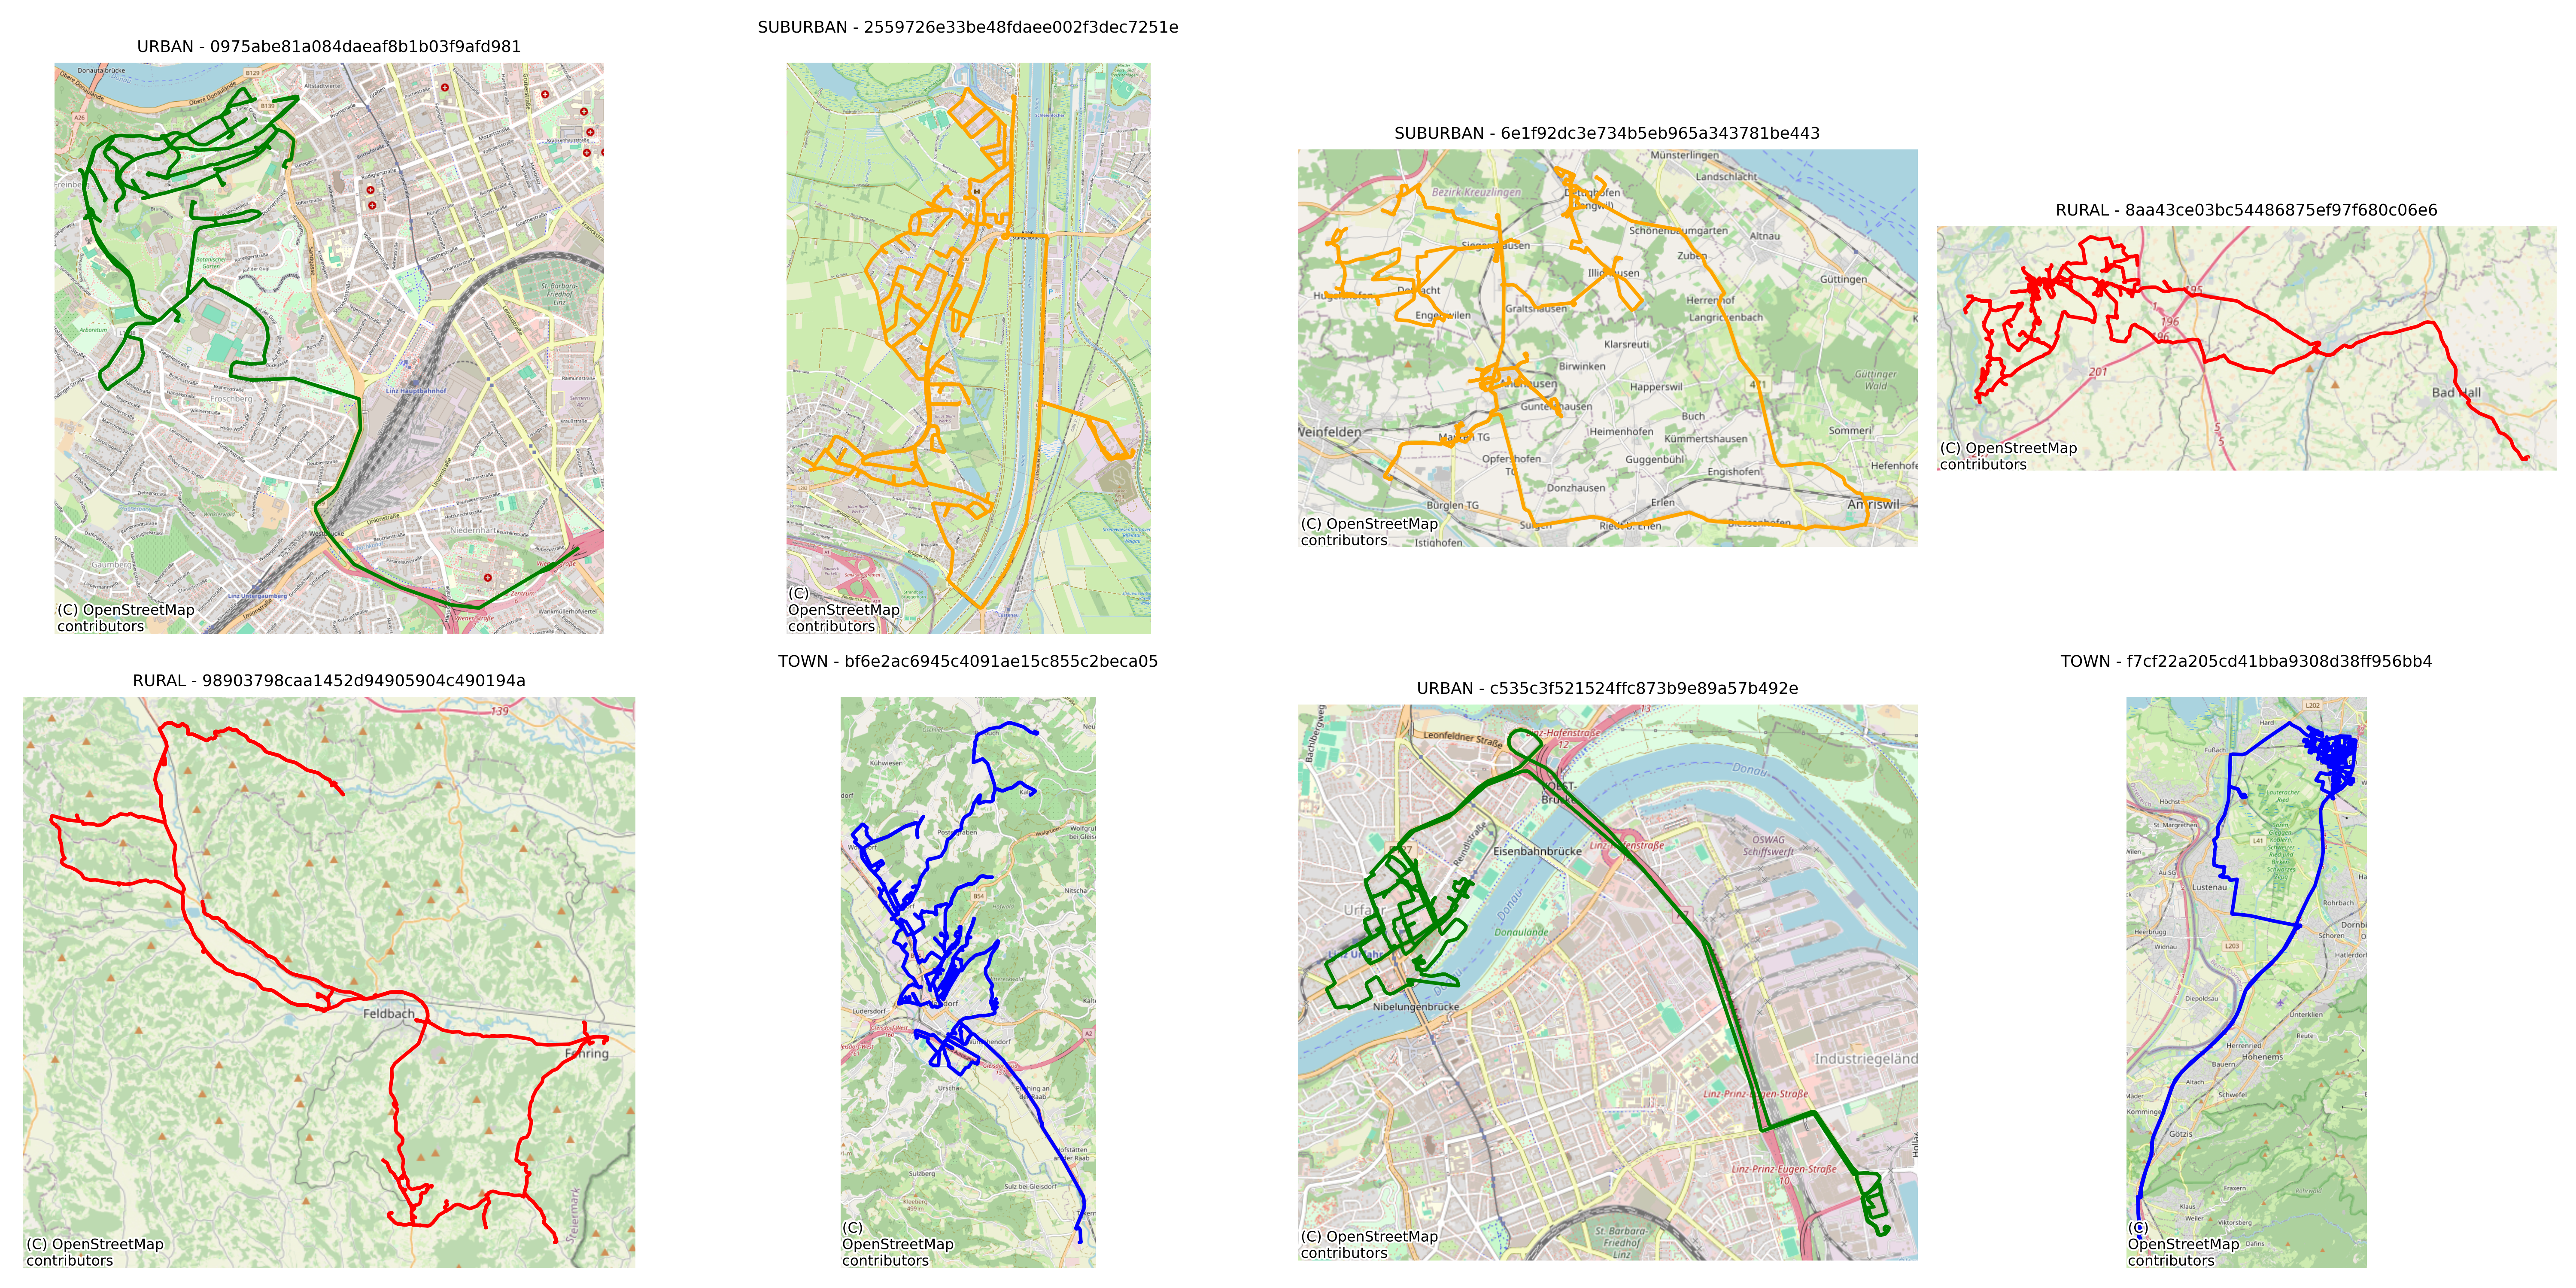
\includegraphics[width=\textwidth]{Figures/sample_tracking_routes_mapgrid.png}
  \caption{Mapgrid for selected sample trackings}
  \label{fig:sample_mapgrid}
\end{figure}
\FloatBarrier
The mapgrid shows spatial layout of each tracking route overlayed on a visual
map. Each subplot corresponds to a single tracking and is colorcoded with the
assigned lable (RURAL=Red, SUBURBAN=Orange, TOWN=Blue, URBAN=Green). This
visual representation clearly shows the difference in route shapes and sizes
between the four different area types.

\textbf{Urban:}
\begin{itemize}
  \item Routes are geographically compact and highly localized.
  \item Movement appears dense with short travel distances between stops.
  \item Often confined to a small cluster of city blocks or neighborhoods.
\end{itemize}

\textbf{Town:}
\begin{itemize}
  \item Coverage is slightly more dispersed than urban routes.
  \item Still relatively compact but less tightly packed.
  \item Serves a central area and nearby residential surroundings.
\end{itemize}

\textbf{Suburban:}
\begin{itemize}
  \item Routes extend farther and cover wider areas than town routes.
  \item Show transitional behavior between urban and rural structures.
  \item Less dense stop distribution, indicating more spaced-out residential
        zones.
\end{itemize}

\textbf{Rural:}
\begin{itemize}
  \item Routes are long and span large geographical areas.
  \item Stops are widely spaced, often connecting small, isolated settlements.
  \item The shape and path vary significantly, often following main roads
        between distant collection points.
\end{itemize}

\begin{figure}[htbp]
  \centering
  \includegraphics[width=\textwidth]{Figures/sample_pairplot.png}
  \caption{Pairplot of selected GPS route features grouped by area label}
  \label{fig:sample_pairplot}
\end{figure}
\FloatBarrier

The pairplot compares the relationships between the extracted features (eg.,
length, duration, number of points, bounding box area, point density, average
segmengt distance and number of stops). Rural and urban trackings show a clear
difference in multiple features. Point density and average segment distance are
especially good discriminators. Suburban and town trackings show more variance
and occasionally overlap with eachother, giving a not so clear distinction.

\begin{figure}[htbp]
  \centering
  \includegraphics[width=\textwidth]{Figures/sample_correlation_matrix.png}
  \caption{Correlation Matrix of selected GPS route features grouped by area
    label}
  \label{fig:sample_correlation_matrix}
\end{figure}
\FloatBarrier

The Correlation Matrix highlights the strong correlations between features in
the selected sample.
A high posive correlation between length, duration and number of points can be
observerd. Additionally the point density has a strong negative correlation
with the tracking length, number of points and average segment distance.

This correlation is to be expected and confirms the consistency of the data,
since the points (GPS coordinates) are recorded in uniform intervals. This plot
also indicates the possible redundance of features such as number of points and
number of stops.

\begin{figure}[h]
  \centering

  \includegraphics[width=\textwidth]{Figures/sample_point_density_boxplot.png}
  \caption{Boxplot of point density grouped by area label}
  \label{fig:sample_boxplot}
\end{figure}
\FloatBarrier

The point density boxplots for each label shows a clear difference between the
labels. Urban trackings appear to have the highest density and rural trackings
the lowest, with suburban and town trackings falling in the middle with a wider
variability.

This validates that the point density is a strong feature for classifying
trackings to the four labels.

\section{Solution Approach}
This chapter outlines the methods used to analyse and classify the GPS tracking
data collected by waste collection vehicles.
The approach is structured in multiple stages, beginning with exploratory data
analysis, proceeding with feature extraction, data cleaning, outlier detection,
clustering and finally training a classifier.
The goal is to identify tracking patterns that allow for structural
classification of trackings into four categories: Urban, Suburban, Town and
Rural.

\subsection{Exploratory Data Analysis}

The foundation of this thesis is the dataset provided by \textit{infeo GmbH}.
It contains anonymized GPS track data collected by waste collection vehicles
during real world operation. Due to its large size of more than 100.000 GPS
tracks and its anonymization, a clear picture of the data needed to be
established as the first step.
With visual examination of different random trackings a sample of eight
manually labeled trackings was gathered.
The selected trackings were labeled to four categories, two trackings per
category.

\begin{itemize}
  \item Urban (Dense building structures, complex road networks, and minimal
        spacing between stops)
  \item Suburban (Moderately spaced residential areas with organized street
        layouts)
  \item Town (Smaller clustered settlements with simpler road structures)
  \item Rural (Sparse housing, long roads, large distances between collection
        points)
\end{itemize}

With the manually selected trackings varying in geographical structure, a
exploratory data
analysis helped transfer the visual distinction to clear differences found in
the data of each tracking category.

\subsection{Feature Extraction from Sample Dataset}
To enable the use of machine learning algorithms, each tracking originally
represented by a consecutive list of GPS waypoints with latitude and longitude
must be transformed into feature vectors. Feature extraction methods were
applied to derive representative metrics for each tracking.

This approach is well established and used in similar studies such as the
classification
of transportation modes by Etemad et al.~\cite{etemad_predicting_2018} and
clustering of GPS data using distance-based features by Koh et
al.~\cite{koh_clustering_2022}

\subsubsection{Features Available in Trackings}

\begin{enumerate}
  \item \textbf{Length:} Total distance of the tracking, in kilometers as
        recorded in the database.
  \item \textbf{Duration:} Total time duration for the tracking, captured and
        recorded in the databse.
\end{enumerate}

\subsubsection{Features Extracted from Waypoints}

\begin{enumerate}
  \item \textbf{Number of Points:} The total number of GPS waypoints recorded
        in the tracking.
  \item \textbf{Bounding Box Area:} The area of the minimum bounding box that
        encloses all latitude and longitude waypoints in one tracking.
  \item \textbf{Point density:} The number of waypoints divided by the bounding
        box area. This feature indicates how closes packed the points are.
  \item \textbf{Average Segment Distance:} The mean distance between
        consecutive waypoints, computed using geodisc distance.
  \item \textbf{Total Distance:} The sum of all segment distances between
        consecutive waypoints. (Later removed, since it is a more unreliable
        length
        metric compared to the length in the tracking metadata)
  \item \textbf{Straightness:} The ratio between the geodesic distance from the
        first to the last point and the total distance of the route. Values
        close to 1
        indicate a straight path, while lower values indicate loops and
        detours.
  \item \textbf{Mean Heading Change:} The average change in bearing between
        consecutive segments of the path, in radians. It reflects how often and
        how
        severe the vehicle changes direction.
  \item \textbf{Number of Stops:} Waypoints with speed of zero. (Later removed,
        due to low variance as most waypoints have a speed of zero)
\end{enumerate}

\subsection{Filtering and Preprocessing the Full Dataset}
There are a lot of faulty datapoints that are not relevant for the
clustering, that are filtered out. Before applying machine learning methods,
extensive filtering was required to
remove invalid and irrelevant data from the dataset. These included:

\begin{enumerate}
  \item Trackings with a too low duration to be realistic collection trackings.

  \item Trackings that recorded movement only in and around a parking lot.
  \item Trackings left running overnight with no significant movement.
  \item Trackings with unrealistic GPS jumps and anomalies (possibly due to
        device errors or compression errors introduced by \textit{infeo GmbH}).
\end{enumerate}

Removing these faulty datapoints was curcial for ensuring the quality of the
clustering and reducing the computation times.

\subsection{Clustering and Pattern Discovery}
To discover patterns in the unlabeled dataset, clustering algorithhms were
applied.
Initially, K-Means++ was used to cluster the data into four clusters. However
the result showed that one cluster mostly consisted of outlier routes, with
unrealistic GPS jumps.

To solve this issue, the process was improved by detecting and removing
outliers using DBSCAN (Density-Based Spatial Clustering for Applications with
Noise). DBSCAN effectively removed most anomalies in the dataset. After
filtering the outliers with DBSCAN, K-Means clustering was applied again,
resulting clusters that represented the four defined categories better.

\subsection{Training a Classification Model}
% TODO: need to write more in this section
To automatically classify new trackings into one of the four categories (Urban,
Suburban, Town, Rural), a supervised machine learning model was trained using
the labeled dataset from the clustering step.
The labeled dataset was split into training and test sets using an 80/20 split.
Evaluation of the classifier on the test set showed a high overall accuracy.
The trained classifier was saved for the later use in a sandbox API to classify
new trackings.

\subsection{API Integration}
To make the trained classification model accessible and usable in a practical
sense, the solution includes the integration of a lightweight REST API.
This enables external systems to send requests to the API endpoint, and
receive a classification result in real-time.
The API is designed to receive a \texttt{tracking\_id} and fetch the tracking
data directly from the \textit{infeo GmbH} platform, preprocess it using the
same logic as the training pipeline, and apply the Random Forest classifier to
return the predicted label.

\section{Structure of the Work}

The remainder of this thesis is structured in the following chapters:

\begin{itemize}
  \item \textbf{Chapter 4: Implementation:} Provides a detailed description of
        how the previously introduced methos and algorithms were implemented.
        This
        includes the data preprocessing, feature extraction, clustering
        pipeline and
        classifier training.
  \item \textbf{Chapter 5: Evaluation and Discussion:} Presents the results of
        the clustering and classification. Performance metrics, visualizations,
        and
        analysis of the results are discussed alongside future reasearch and
        application.
  \item \textbf{Chapter 6: Conclusion:} Summarization of the contributions of
        the thesis, highlighting key takeaways and shortcomings.
\end{itemize}

This structure follows the development of the project, from understanding the
problem and analysing the data, to buildinng and evaluating a solution to
address the objective of classifying GPS trackings into structural categories.
\chapter{Implementation}

This Chapter translates the conceptual pipeline from Chapter 3 into its
concrete Python-based implementation.
Each stage of the pipeline, from data processing to feature extraction,
clustering and classification, was implemented in modular Jupyter Notebooks
using libraries such as \texttt{pandas}, \texttt{scikit-learn}, \texttt{geopy}
and \texttt{pyarrow}.Each module was designed to run independently, allowing
for quick
experimentation and reproducability of results.

% \section{Implementation of the Big Picture}

The
Figure~\ref{fig:big_picture_implemetation_diagram} shows a more detailed view
of the pipeline introduced int Chapter 3.

\begin{figure}[htbp]
  \centering

  \includegraphics[width=0.8\textwidth]{Diagrams/drawio/big_picture_implementation.png}
  \caption{Big picture implementation pipeline}
  \label{fig:big_picture_implemetation_diagram}
\end{figure}
\FloatBarrier

\section{Data Handling and Preprocessing}
Preprocessing is a crucial step in the machine learning pipeline.

Each row in the dataset is a single GPS waypoint and consist of the following
relevant columns:

\begin{itemize}
  \item \textbf{id\_tracking:} Unique identifier for each tracking.
  \item \textbf{sequence:} The order of the waypoint in the tracking.
  \item \textbf{latitude/longitude:} GPS coordinates.
  \item \textbf{speed:} Vehicle speed at the waypoint.
  \item \textbf{tracking\_duration:} Total time of the tracking.
  \item \textbf{tracking\_length:} Total dinstance of the tracking in km.
\end{itemize}

\subsection{Data volume and loading}

The data was provided via a MySQL database, containing two main tables relevant
for this analysis.
Trackings table containing the metadata of 101353 trackings and the waypoints
table containing the corresponding GPS waypoints of the trackings.
Due to the substantial size of database \textbf{~13.5 GB} in total, with
\textbf{~12.6 MB} from the tracking table and \textbf{~11.6 GB} from the
waypoint table,
an efficient data handling pipeline was necessary.

To handle the data at a lower scale, the filtering query was executed directly
within the database using SQL (see Listing~\ref{lst:sql-filter}). The resulting
filtered dataset was streamed in chunks of \texttt{1,000,000} rows using
\texttt{pandas.read\_sql()} and saved incrementally to a compressed Apache
Parquet file using \texttt{pyarrow}. The final Parquet file had a reduced size
of approximately \textbf{1.5 GB}.

This chunk-wise approach ensured memory efficient loading without crashing the
kernel with the limited hardware available.
The full export operation took about two hours to fully complete, with an
average processing speed of \texttt{6.40 iterations/second} (row group read and
write cycles).

\subsection{Filtering Faulty Trackings}
The raw data included many invalid or irrelevant trackings that could impact
the analysis and clustering. These trackings were removed based on these
criteria:

\begin{itemize}
  \item \textbf{Duration Filter:} Trackings shorter than 30 minutes or longer
        than 10 hours were excluded.
  \item \textbf{Length Filter:} Trackings with a total length lower than 50 km
        or above 850km were excluded.
  \item \textbf{Minimal Waypoint Count:} Trackings with less than 10 recorded
        waypoints were excluded.
  \item \textbf{Minimal Bounding Box:} Trackings with a bounding box smaller
        than about 50 meters in latitude or longitude were excluded. This was a
        helpful
        step to reduce the amount of trackings that were exclusively recorded
        in a
        parking lot.
\end{itemize}

The filters were directly implemented as a SQL query executed in an jupyter
notebook. This reduced the further computatinal times for clustering and
training the classifier model. The SQL query implementing these filters looked
as follows:
\begin{lstlisting}[style=sql,caption={SQL query used for filtering the GPS tracking dataset},label={lst:sql-filter}]
  SELECT 
      wp.id_tracking, wp.id, wp.time, wp.type, wp.sequence, wp.comment, 
      wp.speed, wp.heading, wp.duration, wp.block_type, wp.log, 
      wp.latitude, wp.longitude, wp.altitude, wp.meta_tag, wp.meta_value,
      t.length AS tracking_length, 
      t.duration AS tracking_duration
  FROM waypoint wp
  JOIN tracking t ON wp.id_tracking = t.id
  WHERE 
      t.duration BETWEEN 18000000000 AND 360000000000  
      -- 0.5 to 10 hours
      AND t.length BETWEEN 50 AND 850  -- 50 to 850 km
      AND EXISTS (
          SELECT 1 FROM waypoint w 
          WHERE w.id_tracking = t.id
          HAVING COUNT(*) > 10  -- Min. 10 waypoints
      )
      AND (
          (SELECT MAX(latitude) FROM waypoint WHERE id_tracking = t.id) - 
          (SELECT MIN(latitude) FROM waypoint WHERE id_tracking = t.id)
      ) > 0.0005  -- Min. ~50m latitude span
      AND (
          (SELECT MAX(longitude) FROM waypoint WHERE id_tracking = t.id) - 
          (SELECT MIN(longitude) FROM waypoint WHERE id_tracking = t.id)
      ) > 0.0005;  -- Min. ~50m longitude span
  \end{lstlisting}

Each Filter step reduces the dataset by this many trackings:
\begin{table}[ht]
  \centering
  \begin{tabular}{|l|r|r|r|}
    \hline
    \textbf{Filter Step}     & \textbf{Remaining Trackings} &
    \textbf{Removed}
                             &
    \textbf{Reduction (\%)}
    \\
    \hline
    All trackings            & 101353                       & --
                             & --
    \\
    Duration filter          & 66477                        &
    34876
                             &
    34.410\%
    \\
    Length filter            & 45668                        &
    20809
                             &
    31.303\%
    \\
    Minimal Waypoints filter & 45599                        &
    69
                             &
    0.151\%
    \\
    Min Lat/Long span filter & 45598                        &
    1
                             &
    0.002\%
    \\
    \hline
    \textbf{Total Remaining} & \textbf{45598}               &
    \textbf{55755}
                             &
    \textbf{55.011\%}
    \\
    \hline
  \end{tabular}
  \caption{Tracking reduction per filtering step}
  \label{tab:filtering_summary}
\end{table}
\FloatBarrier

\section{Feature Extraction}
TODO: small text for section

This section describes how raw GPS tracking data was transformed into
meaningful features that enable the use of machine learning methods in later
steps.
The features were selected based on literature and domain knowledge to capture
the characteristics of the waste collection routes.
The resulting features were used for clustering and for training the supervised
classifier. Each feature was extracted using Python libraries such as
\texttt{pandas}, \texttt{numpy}, and \texttt{geopy} and stored in a CSV file.

\subsection{Available Metadata Features}

Metadata features are directly provided in the dataset for each tracking. They
serve as a
baseline for route length and duration.

\paragraph{Tracking length}
The total recorded travel distane in kilometers, as stored in the metadata.

\paragraph{Tracking duration}
The full duration from the first to the last recorded waypoint, in
100-nanosecond intervals.

\subsection{Computed Features from Waypoints}
TODO: small text for subsection
These features are derived from the sequence of waypoint for each tracking.
They enrich the metadata by describing the geometry and dynamics of each
tracking.
All calculations were implemented using the \texttt{geopy} library for geodesic
distances and \texttt{numpy} for vectorized operations.
The most relevant features are described below.

\paragraph{Number of points}

The total number of waypoints $n$ in a tracking:
\[
  num\_points = n
\]

\paragraph{Bounding box area}

Computed from the geodesic height $h$ and width $w$ of the minimal enclosing
rectangle:
\[
  bbox\_area = h \cdot w
\]
\[
  h = d((lat_{\min}, long_{\min}), (lat_{\max}, long_{\min})), \quad w =
  d((lat_{\min}, lon_{\min}), (lat_{\min}, long_{\max}))
\]
where $d(\cdot, \cdot)$ refers to the geodesic distance between two GPS points
(in
meters), calculated using the WGS84 ellipsoid model through the \textit{geopy}
Python library~\cite{noauthor_welcome_nodate}.

\paragraph{Point density}

Density of GPS waypoints in the bounding box:
\[
  point\_density = \frac{n}{bbox\_area + \varepsilon}, \quad
  \varepsilon = 10^{-6}
\]
where $\varepsilon$ is a small constant to avoid division by zero.

\paragraph{Average segment distance}

The average geodesic distance between consequtive waypoints:
\[
  avg\_segment\_distance = \frac{1}{n-1} \sum_{i=1}^{n-1} d(p_i, p_{i+1})
\]
where $d(\cdot, \cdot)$ refers to geodesic distance.

\paragraph{Total Distance}
The cumulative travel distance:
\[
  total\_distance = \sum_{i=1}^{n-1} d(p_i, p_{i+1})
\]

\paragraph{Straightness}
Ratio between the start-end distance and the total path length:
\[
  straightness = \frac{d(p_1, p_n)}{\sum_{i=1}^{n-1} d(p_i, p_{i+1})}
\]
~\cite{benhamou_how_2004}

\paragraph{Mean Heading Change}
Average angle change between consecutive direction vectors (in radians):
\[
  \delta_i = \min(|\theta_{i+1} - \theta_i|, 2\pi - |\theta_{i+1} - \theta_i|),
  \quad
  mean\_heading\_change = \frac{1}{n-2} \sum_{i=1}^{n-2} \delta_i
\]
with bearings $\theta_i$ computed via:
\[
  \theta = \arctan2\left( \sin(\Delta \lambda) \cos(\phi_2),
  \cos(\phi_1)\sin(\phi_2) - \sin(\phi_1)\cos(\phi_2)\cos(\Delta \lambda)
  \right)
\]
~\cite{etemad_predicting_2018}

\paragraph{Number of Stops}
Amount of waypoints where the truck had a speed of zero:
\[
  num\_stops = \sum_{i=1}^{n} \mathbb{1}(speed_i = 0)
\]

\subsection{Feature Storage and Output}

The extracted features were stored in a structured CSV file, with one row per
tracking and all corresponding features. This resulting dataset forms the
basis for all future analysis, clustering and classification applications in
the next steps of the pipeline.

\begin{table}[ht]
  \centering
  \begin{tabular}{|l|l|l|}
    \hline
    \textbf{Feature}                & \textbf{Unit} & \textbf{Description}
    \\
    \hline
    \texttt{num\_points}            & Count         & Number of GPS waypoints
    in a tracking
    \\
    \texttt{bbox\_area}             & $m^2$         & Area of bounding box
    enclosing all GPS points
    \\
    \texttt{point\_density}         & points/m$^2$  & Number of points per
    square meter
    of bounding box
    \\
    \texttt{avg\_segment\_distance} & m             & Mean geodesic distance
    between
    consecutive waypoints
    \\
    \texttt{total\_distance}        & m             & Total geodesic distance
    covered by the
    tracking
    \\
    \texttt{straightness}           & Ratio (0–1)   & Direct distance from
    start to end /
    total distance
    \\
    \texttt{mean\_heading\_change}  & rad           & Average absolute angle
    change
    between segments
    \\
    \texttt{num\_stops}             & Count         & Number of waypoints with
    speed = 0
    \\
    \texttt{duration}               & 100 ns        & Total tracking
    duration in nanoseconds
    \\
    \texttt{length}                 & km            & Total tracking length
    from the database
    \\
    \hline
  \end{tabular}
  \caption{Extracted features with units and descriptions}
  \label{tab:feature_units}
\end{table}

\section{Clustering Implementation}

% \begin{figure}[htbp]
%   \centering

%   \includegraphics[width=1\textwidth]{Figures/histogram_feature_data_pre_clustering.png}
%   \caption{Histogram}
%   \label{fig:histogram-feature-engineered-data}
% \end{figure}
% \FloatBarrier

% \begin{figure}[htbp]
%   \centering

%   \includegraphics[width=1\textwidth]{Figures/correlation_matrix_pre_clustering.png}
%   \caption{Correlation matrix}
%   \label{fig:correlation-matrix}
% \end{figure}
% \FloatBarrier

\subsection{Outlier Removal with DBSCAN}

% doesnt belong here (goes down to evaluation)
% \begin{figure}[htbp]
%   \centering

%   \includegraphics[width=0.9\textwidth]{Figures/dbscan_diagram_feature_data.png}
%   \caption{DBSCAN}
%   \label{fig:dbscan-clustering-outlier-removal}
% \end{figure}
% \FloatBarrier

\subsection{Semi-Supervised Clustering with Weighted and Seeded K-Means}

% TODO: Rewrite this entire section -> 100% AI 

To improve the interpretability and performance of clustering, a
semi-supervised approach was used to guide the K-Means algorithm. A manually
labeled subset of 8 samples, evenly distributed across the four target
categories (\texttt{URBAN}, \texttt{SUBURBAN}, \texttt{TOWN}, \texttt{RURAL}),
was utilized to derive feature weights and initialize cluster centroids. This
allowed the unsupervised clustering algorithm to be seeded with domain
knowledge.

\begin{figure}[htbp]
  \centering

  \includegraphics[width=0.9\textwidth]{Diagrams/drawio/implementation/clustering_pipeline.png}
  \caption{K-Means semi supervised clustering pipeline}
  \label{fig:kmeans-clustering-pipline}
\end{figure}
\FloatBarrier

\subsubsection{Feature Weighting Based on Sample Label Spread}

In order to emphasize features that varied significantly across known classes
and downweight features with less discriminative power, relative variability of
feature medians between the categories was used. Specifically, for each feature
$f_i$, the relative median range was calculated as:

\[
  w_i = \frac{max_i - min_i}{mean_i}
\]

where $max_i$, $min_i$, and $mean_i$ represent the
maximum, minimum, and mean median value of feature $f_i$ across the four
labeled classes. These weights were then normalized by dividing by the mean of
all $w_i$ to ensure comparability:

\[
  w_i^{norm} = \frac{w_i}{\frac{1}{n}\sum_{j=1}^n w_j}
\]

Finally, the weights were clipped to the range $[0.5, 2.0]$ to avoid extreme
scaling effects ~\cite{guyon_introduction_nodate}.

\subsubsection{Seeded Cluster Initialization}

The cluster centers were initialized using the scaled and weighted medians of
the labeled sample set. For each class, the feature medians were calculated,
scaled using the \texttt{StandardScaler}, and then multiplied by the learned
feature weights. The resulting $4 \times d$ matrix was used to seed the $k$
centroids of the K-Means algorithm:

\[
  \mu_k = scale(median_k) \cdot w_i^{norm}
  \quad for each k \in \{1, 2, 3, 4\}
\]

This strategy ensured that the initial centroids already reflected meaningful
differences in the data as identified by the sample set.

\subsubsection{Constrained K-Means Clustering}

The clustering was performed using the \texttt{KMeansConstrained} algorithm
with the following configuration:

\begin{itemize}
  \item Number of clusters: 4
  \item Initialization: Manual (from scaled, weighted medians)
  \item Minimum cluster size: 5\% of total data
  \item Maximum cluster size: 60\% of total data
  \item Number of restarts: 10
\end{itemize}

This method produced clusters that closely aligned with the known class
distribution and improved the stability and interpretability of the clustering
outcome compared to random initialization.

\section{Classification Model}
% TODO: Rewrite entire section -> written 100% by AI
To predict the category of new or unlabeled GPS trackings, a classification
model was trained using the extracted and clustered features. A Random Forest
classifier was chosen due to its robustness, ability to handle high-dimensional
data, and interpretability via feature importance.

\subsection{Model Selection and Training}

The full labeled dataset, enriched with cluster labels from the K-Means
process, was split into a training and a test set using a 2:1 ratio. A grid
search with 3-fold cross-validation was performed to identify the best
hyperparameters for the Random Forest model. The following parameter grid was
used:

\begin{itemize}
  \item Number of estimators: \texttt{[100, 200, 300]}
  \item Maximum depth: \texttt{[10, 15, 20]}
  \item Minimum samples split: \texttt{[2, 5]}
  \item Minimum samples leaf: \texttt{[1, 2]}
  \item Class weight: \texttt{[None, 'balanced']}
\end{itemize}

The best model was found with 300 trees, a maximum depth of 20, and default
class weights. The model achieved an accuracy of
98.3\% on the test set.

% \subsection{Model Evaluation}

% The classifier was evaluated using standard metrics:

% \begin{itemize}
%   \item \textbf{Accuracy:} 0.983
%   \item \textbf{Macro F1-score:} 0.981
%   \item \textbf{Weighted F1-score:} 0.983
%   \item \textbf{Cohen's Kappa:} High agreement with actual labels
% \end{itemize}

% A confusion matrix and class distribution bar plots were created to assess
% prediction quality. All classes were well-separated with minimal confusion. The
% silhouette score of -0.1393, although typical for high-dimensional data,
% reflects some overlap near decision boundaries.

% \subsection{Feature Importance Analysis}

% The feature importance plot revealed which GPS tracking characteristics had the
% strongest influence on classification. The most informative features included
% bounding box area, point density and length.

% SHAP (SHapley Additive exPlanations) values were also computed to explain
% individual predictions. Global and per-class SHAP summary plots confirmed the
% consistency of the feature contributions with domain expectations.

% \subsection{Prediction Analysis and Visualization}

% Several visual analyses were performed on the test set:

% \begin{itemize}
%   \item \textbf{Boxplots} showing feature distribution across predicted labels
%   \item \textbf{Normalized heatmaps} comparing average feature values per
%         predicted class
%   \item \textbf{PCA scatterplot} visualizing predicted clusters in 2D space
%   \item \textbf{Geographic maps} of randomly sampled predicted routes for each
%         label
% \end{itemize}

% These visualizations support that the classifier not only performs well
% statistically but also produces geographically and behaviorally consistent
% results.

\subsection{Saving and Exporting the Classifier}

The trained Random Forest model was serialized using \texttt{joblib} and
exported as a \texttt{.pkl} file. This model can be directly
integrated into production pipelines or reused for further research.
Predictions from the classifier were stored for visualization and evaluation
purposes in a CSV file.

% \subsection{Cross-Validation Results}

% To validate model stability, 10-fold stratified cross-validation was applied to
% the full dataset. The mean accuracy across folds was approximately
% 98\% with a very low standard deviation, confirming the generalizability of the
% classifier.

\subsection{Conclusion}

The Random Forest classifier achieved high performance and provided
interpretable insights into how GPS tracking data reflects urban, suburban,
town, and rural driving patterns. The combination of clustering,
semi-supervised learning, and explainable machine learning techniques created a
robust
classification pipeline for real-world tracking analysis.

\section{Integration with API}

To provide real-time classification, a FastAPI-based web service was
implemented (Figure~\ref{fig:fastapi_implementation_diagram}). The service
exposes a single endpoint which takes a
\texttt{tracking\_id} as an input, fetches the corresponding tracking data from
the \textit{infeo GmbH} API, and processes the tracking data through the same
preprocessing pipeline used during the model training.

The API loads the trained classifier from a serialized \texttt{.pkl} file and
predicts the label of processed tracking.
The endpoint then returns the \texttt{tracking\_id} and the predicted class
label in a \textit{json} format.

Figure~\ref{fig:fastapi_docs} shows the automatically generated \textit{Swagger
  UI} documentation of the endpoint.

\begin{figure}[htbp]
  \centering

  \includegraphics[width=0.9\textwidth]{Diagrams/drawio/api/api_implementation.png}
  \caption{API Implementation Diagram}
  \label{fig:fastapi_implementation_diagram}
\end{figure}

\begin{figure}[htbp]
  \centering

  \includegraphics[width=0.9\textwidth]{Figures/api/fastapi_documentation.png}
  \caption{Swagger UI documentation of FastAPI Classification Endpoint}
  \label{fig:fastapi_docs}
\end{figure}

\chapter{Evaluation and Discussion}
% TODO: EXpertenmeinung zu den ergebnissen der classification von florian einbauen (evtl eigene section)

This chapter presents a comprehensive evaluation of the clustering and
classification results.
It provides insights into the performance, limitations, and robustess of the
developed system.

\section{Definition of the data sets used for the evaluation}

To assess the quality of the clustering and classification steps, various
datasets at different stages of the pipeline were used.
The final labeled dataset was split into training and test sets using a 2:1
ratio to evaluate the classifier's generalization ability.

\section{Evaluation of the Results}

\subsection{Clustering Results}

The DBSCAN clustering algorithm was used to remove noise points and outliers,
resulting in the removal of 1,539 trackings.
The PCA projection in Figure~\ref{fig:pca_dbscan} shows the detected outlier
cluster (-1), sbusequently removed resulting in a cleaner structure for the
K-Means clustering.

\begin{figure}[htbp]
  \centering

  \includegraphics[width=0.9\textwidth]{Figures/dbscan_diagram_feature_data.png}
  \caption{PCA Projection of DBSCAN clustering for noise removal}
  \label{fig:pca_dbscan}
\end{figure}
\FloatBarrier

The feature weights calulated from the manually selected sample data showed
that \texttt{bbox\_area}, \texttt{point\_density},
\texttt{straigthness} and \texttt{length} were the most informative features.
The concrete values are depipicted
in Figure ~\ref{fig:feature_weights_for_kmeans}.

Weighted K-Means clustering with custom initial centroids produced four
distinct clusters. Each cluster was mapped to a label (\texttt{0-URBAN},
\texttt{1-SUBURBAN}, \texttt{2-TOWN}, \texttt{3-RURAL}) based on feature
statistic and visual inspection.
The PCA projection in Figure ~\ref{fig:pca_kmeans} visualized the resulting
cluster structure, with a final silhouette score of \textbf{0.2621} indicates a
moderate clustering
separation.

\begin{figure}[htbp]
  \centering

  \includegraphics[width=0.9\textwidth]{Figures/feature_weights.png}
  \caption{Feature Weights used for K-Means clustering}
  \label{fig:feature_weights_for_kmeans}
\end{figure}

\begin{figure}[htbp]
  \centering

  \includegraphics[width=0.9\textwidth]{Figures/kmeans_diagram_feature_data.png}
  \caption{PCA Projection of K-Means clustering}
  \label{fig:pca_kmeans}
\end{figure}
\FloatBarrier

\begin{figure}[htbp]
  \centering

  \includegraphics[width=0.9\textwidth]{Figures/classifier/shap_summary_for_all_classes.png}
  \caption{SHAP Summary for all Classes}
  \label{fig:shap_all_classes}
\end{figure}

% map visualization of clustered trackings by K-Means
\begin{figure}[p]
  \centering

  \begin{subfigure}[b]{0.495\textwidth}
    \centering

    \includegraphics[width=\textwidth]{Figures/clustering_map/clustering_result_map_rural_area1.png}
    \caption{Lower Bavaria}
    \label{fig:clustering_map_visulaization_rural}
  \end{subfigure}
  \hfill
  \begin{subfigure}[b]{0.495\textwidth}
    \centering

    \includegraphics[width=\textwidth]{Figures/clustering_map/clustering_result_map_konstanz_area_town1.png}
    \caption{Thurgau: Kreuzlingen and Konstanz}
    \label{fig:clustering_map_visulaization_konstanz}
  \end{subfigure}

  \vspace{1cm}

  \begin{subfigure}[b]{0.495\textwidth}
    \centering

    \includegraphics[width=\textwidth]{Figures/clustering_map/clustering_result_map_linz_urban1.png}
    \caption{Upper Austria: Linz}
    \label{fig:clustering_map_visulaization_linz}
  \end{subfigure}
  \hfill
  \begin{subfigure}[b]{0.495\textwidth}
    \centering

    \includegraphics[width=\textwidth]{Figures/clustering_map/clustering_result_map_vorarlberg_closeup.png}
    \caption{Vorarlberg}
    \label{fig:clustering_map_visulaization_vorarlberg}
  \end{subfigure}

  \caption{Map Visualization of Clustered Trackings (Red: \texttt{URBAN},
    Orange: \texttt{SUBURBAN}, Blue: \texttt{TOWN}, Green: \texttt{RURAL})}
  \label{fig:clstering_map_visualizations}
\end{figure}
\FloatBarrier

\subsection{Classifier Results}

A Random Forest classifier was trained with hyperparameter tuning.
The model achieved high performance on the test set: Accuracy \textbf{98.3\%},
Macro F1-score: \textbf{98.1\%}, Weighted F1-score \textbf{98.3\%} and Cohen's
Kappa \textbf{97.3\%}.
The classifier showed balanced performance across all four classes, with
precision and recall values above \textbf{97\%} for all classes.

The feature importance analysis (Figure
~\ref{fig:feature_importance_random_forest})
highlighted \texttt[length], \texttt{bbox\_area}, \texttt{point\_density} and
\texttt{num\_points} as key contributing features.

\begin{figure}[htbp]
  \centering

  \includegraphics[width=0.9\textwidth]{Figures/classifier/confusion_matric_label_prediction.png}
  \caption{Confusion Matrix of Random Forest Classifier}
  \label{fig:confusion_matrix_random_forest}
\end{figure}

\begin{figure}[htbp]
  \centering

  \includegraphics[width=0.9\textwidth]{Figures/classifier/feature_importance_random_forest.png}
  \caption{Feature Importance Barchart of Random Forest Classifier}
  \label{fig:feature_importance_random_forest}
\end{figure}

The mean feature values across all four classes (Figure
~\ref{fig:mean_feature_value_matrix_by_class}) confirm a monotonic
relationships
between classes in increasing rurality (e.g.,\texttt{URBAN} to
\texttt{SUBURBAN} to \texttt{TOWN} to
\texttt{RURAL})
for the features
\texttt{bbox\_area}, \texttt{point\_density}, \texttt{avg\_segment\_distance}
and \texttt{length}.

\begin{figure}[htbp]
  \centering

  \includegraphics[width=0.9\textwidth]{Figures/classifier/feature_values_normalized.png}
  \caption{Normalized Mean Feature Values by Predicted Class}
  \label{fig:mean_feature_value_matrix_by_class}
\end{figure}
\FloatBarrier

\begin{figure}[htbp]
  \centering

  \includegraphics[width=0.9\textwidth]{Figures/classifier/pca_projection_test_set.png}
  \caption{PCA Projection of Test Set with Predicted Labels}
  \label{fig:pca_projection_test_set}
\end{figure}
\FloatBarrier

\begin{figure}[htbp]
  \centering

  \includegraphics[width=0.9\textwidth]{Figures/classifier/shap_summary_for_all_classes.png}
  \caption{SHAP Summary for all Classes}
  \label{fig:shap_all_classes}
\end{figure}

\begin{figure}[p]
  \centering

  \begin{subfigure}[b]{0.495\textwidth}
    \centering

    \includegraphics[width=\textwidth]{Figures/classifier/shap/shap_summary_for_URBAN.png}
    \caption{Urban}
    \label{fig:shap_urban}
  \end{subfigure}
  \hfill
  \begin{subfigure}[b]{0.495\textwidth}
    \centering

    \includegraphics[width=\textwidth]{Figures/classifier/shap/shap_summary_for_SUBURBAN.png}
    \caption{Suburban}
    \label{fig:shap_suburban}
  \end{subfigure}

  \vspace{1cm}

  \begin{subfigure}[b]{0.495\textwidth}
    \centering

    \includegraphics[width=\textwidth]{Figures/classifier/shap/shap_summary_for_TOWN.png}
    \caption{Town}
    \label{fig:shap_town}
  \end{subfigure}
  \hfill
  \begin{subfigure}[b]{0.495\textwidth}
    \centering

    \includegraphics[width=\textwidth]{Figures/classifier/shap/shap_summary_for_RURAL.png}
    \caption{Rural}
    \label{fig:shap_rural}
  \end{subfigure}

  \caption{SHAP summary plots for all classes}
  \label{fig:shap_all_classes}
\end{figure}

Finally four random trackings from each category were selected from the
classified test set and visualized on map segments
~\ref{fig:four_final_predictions_on_testset}, validating the structural and
spatial differences of the labels.

\begin{figure}[htbp]
  \centering

  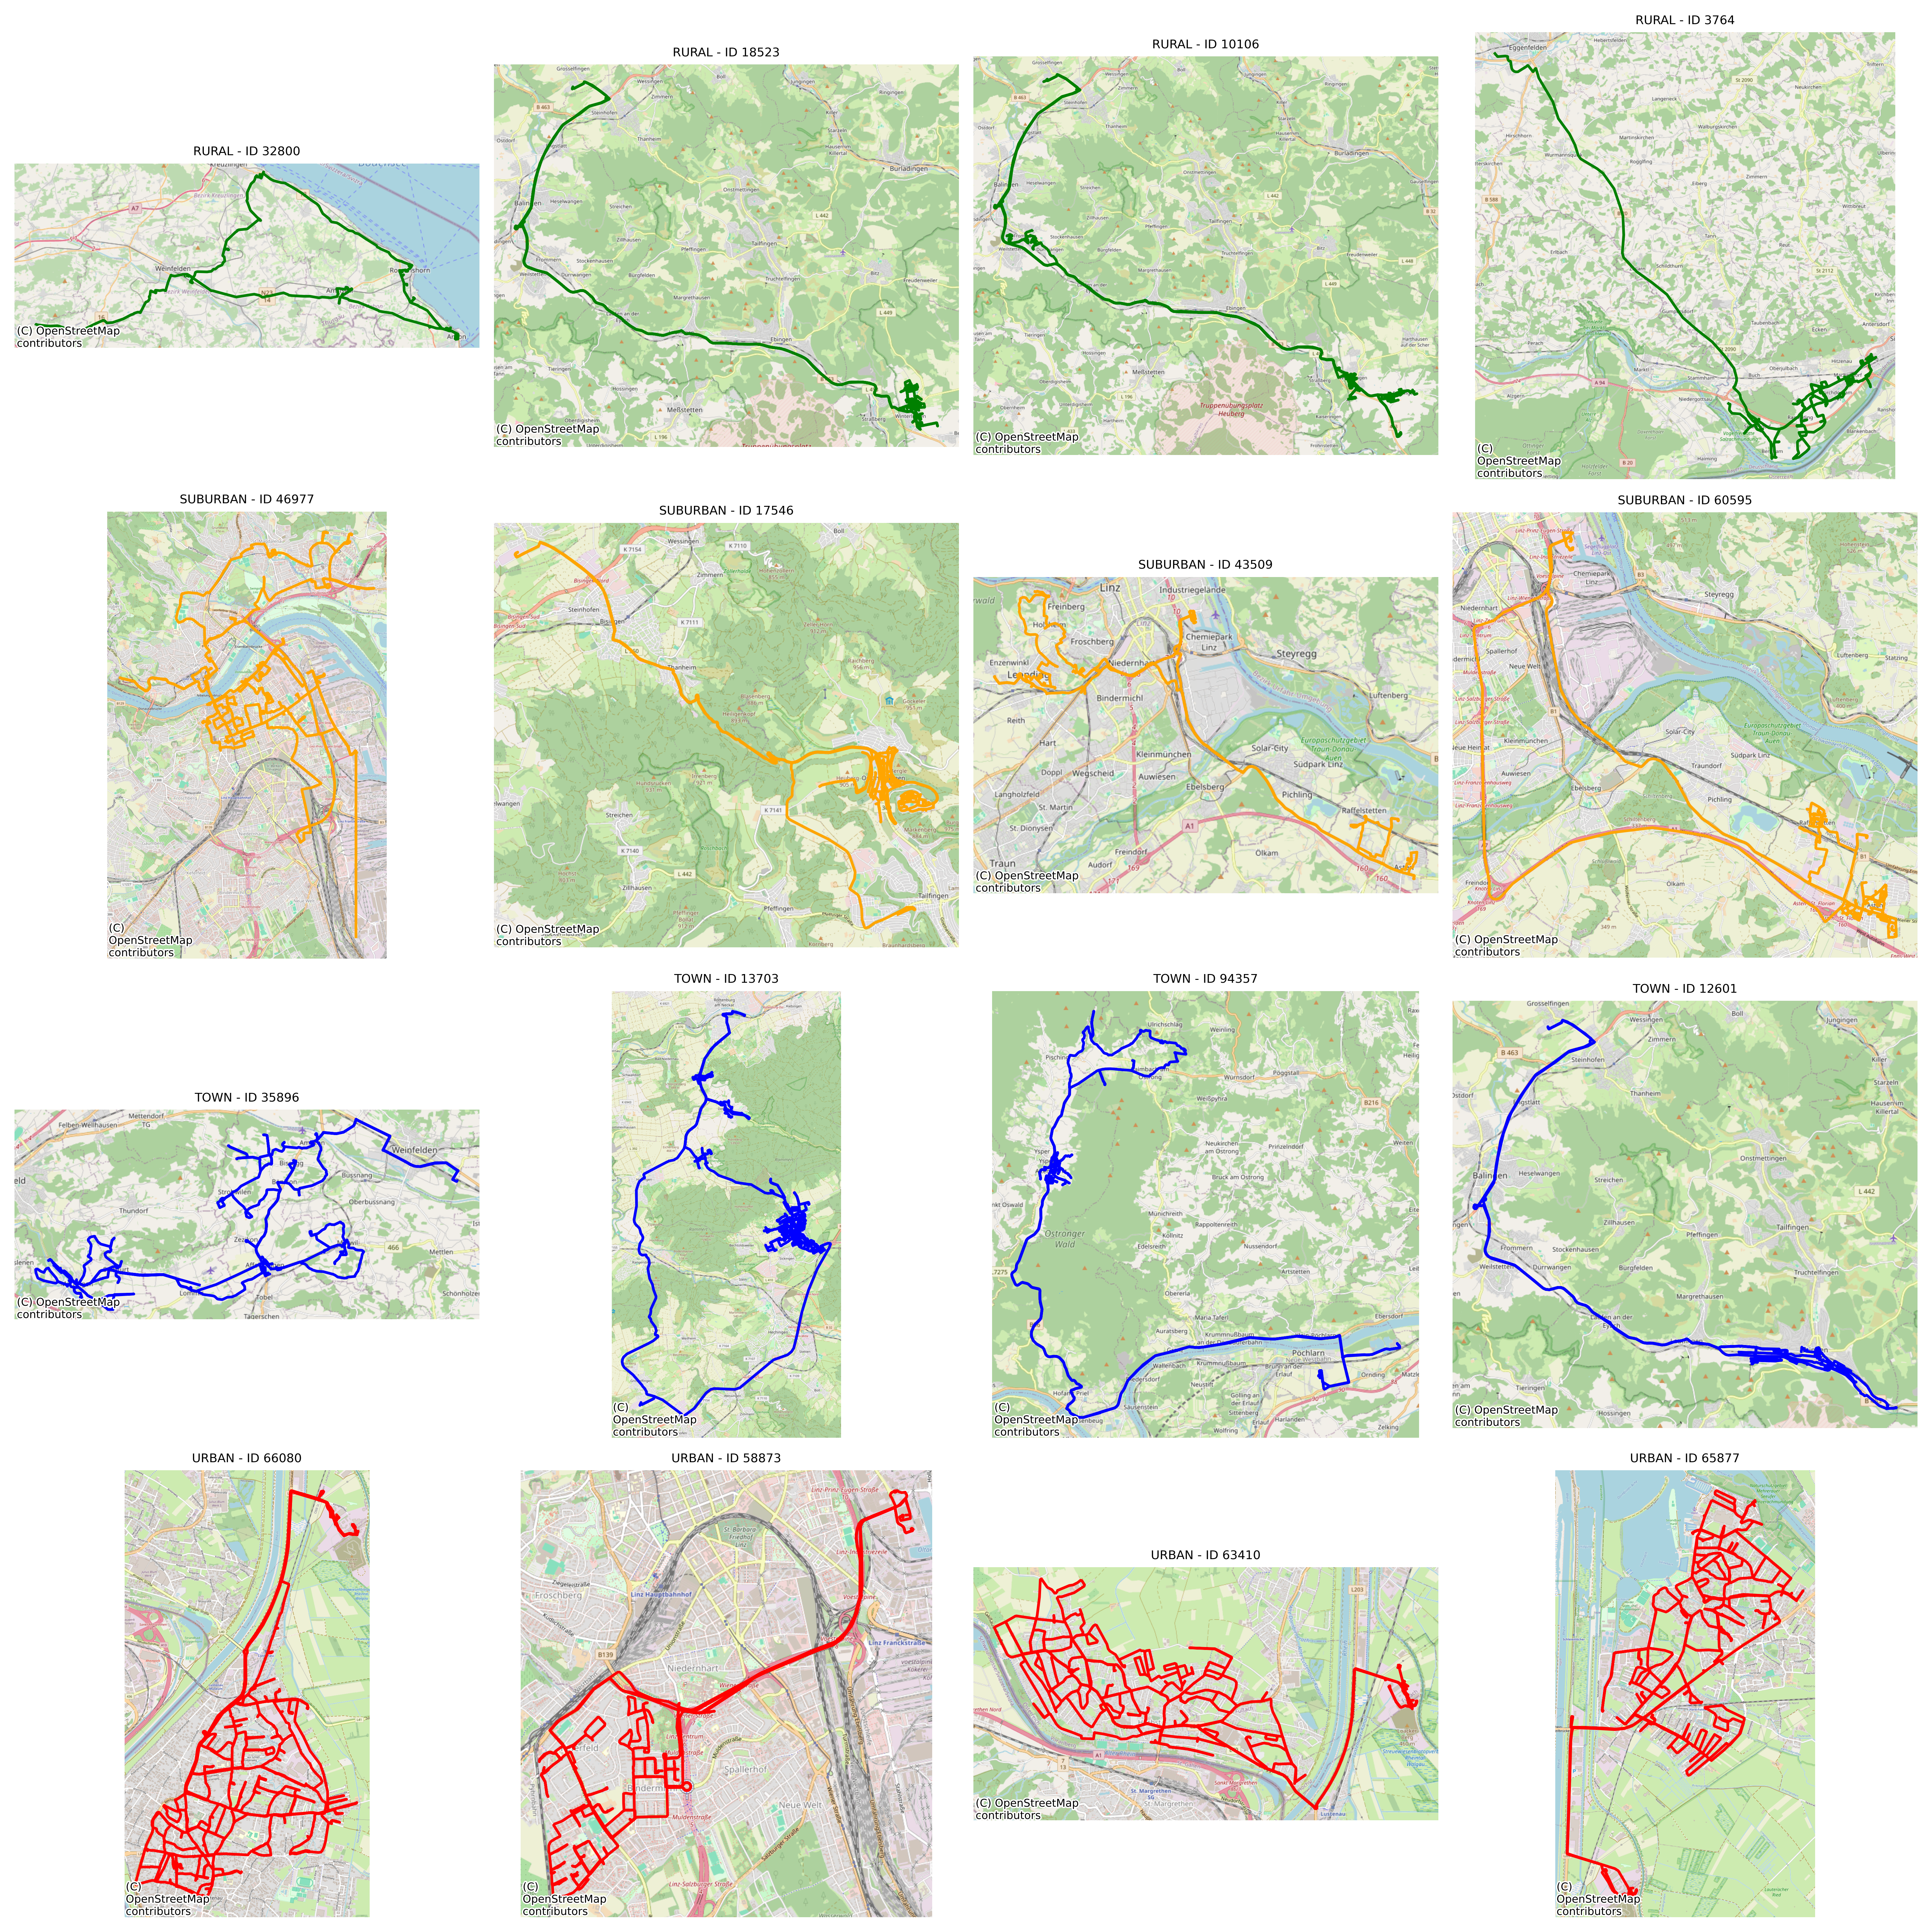
\includegraphics[width=\textwidth]{Figures/classifier/four_final_predictions_per_class.png}
  \caption{Sample Predictions on Test Set}
  \label{fig:four_final_predictions_on_testset}
\end{figure}
\FloatBarrier

\section{Reflection on the Results}

The clustering and classification pipeline effectively distinguishes between
urban structures based on GPS tracking data, with the classifier achieving high
accuracy with over \textbf{97\%} in all
key metrics. While the clustering silhouette score was moderate, visual and
statistical inspection validate the coherence of the clusters.

Despite the promising results, some limitations of the evaluation setup must be
considered. The classifier was trained and tested using labels generated
through semi-supervised K-Means clustering. While the clustering was guided by
meaningful initial centroids and validated visually and statistically, the
resulting labels do not represent objective ground truth. Consequently, the
classifier's high accuracy of \textbf{98.3\%} reflects strong alignment with
the underlying clustering logic rather than verified real-world
classifications. The model has yet to be validated against expert-labeled or
GIS-based reference data, and its generalizability beyond the current dataset
remains an open question.

The negative silhouette score on the test set shows some significant
overlap between classes in the high-dimensional space. This could
be adressed in future iterations by reducing te number of clusters (e.g.,
merging \texttt{SUBURBAN} and \texttt{TOWN}) or by incorporating additional
features from OpenStreetMap.

The features \texttt{bbox\_area}, \texttt{point\_density} and
\texttt{duration},
initally deemed suitable for distinction between classes, because of their
motonic
behavior, were confirmed to be indicative discriminators.
Furthermore, the
classification results show that \texttt{avg\_segment\_distance} and
\texttt{mean\_heading\_change} also follow motonic behavior among classes,
reinforcing the efficteveness of this pipeline.

Overall, the presented method offers a reproducible and scalable approach for
GPS-based
route classification, with potential applications in waste collection
planning, infrastructure analysis, and beyond. With further validation and
integration of additional geospatial data, the framework has the potential to
evolve into a robust decision support tool.

\chapter{Conclusion}

This thesis demonstrates that it is feasible to classify the structure of road
networks
using only GPS tracking data collected by waste collection vehicles.
A robust pipeline to categorize trackings into four distinct urban structure
types: \texttt{URBAN}, \texttt{SUBURBAN}, \texttt{TOWN} and \texttt{RURAL} was
developed using feature engineering, semi-supervised clustering, and supervised
classification.

\section{Future Directions}

Several opportunities exist to improve and extend this thesis.

One promising direction involves the integration of OpenStreetMap (OSM) data to
augment the GPS based features with real-world structural information. On the
one hand this could improve the classifier's ability to differentiate between
trackings with similar GPS structure, while on the other hand enabling the
comparison with areas where no data is collected.

Additionally, enhancing the preprocessing pipeline with a filter to remove
transit segmets between depots and services areas in the trackings can focus
the
analysis on the actual waste collection behavior.

Improving the selected sample for the semi-supervised clustering process, both
in terms of amount and variation of manually labeled trackings
could improve the feature weights and initial centroids heavily affecting the
clustering process.

Finally, deploying the trained clasifier as a REST API, would enable
waste management companies to automatically classify GPS trackings in
real-time,
potentially enabling smarter planning, anomaly detection, and route
optimization.

\section{Limitations}

Despite the promising results of the classification pipeline, several
limitations must be acknoladged.

Firstly, the dataset used in this thesis is not raw GPS data but rather a
compressed and preprocessed version provided by \textit{infeo GmbH}.
While this process is necessary for storage and performance, it might have
removed information that could improve the clustering and classification
accuracy and reveal more fine grained distinction between the categories.

Secondly, while the dataset provides accurate GPS coordinates, the metadata is
limited or unreliable. Attributes such as speed are missing entirely, and
loading and
unloading events were only sparsely available. As a result only GPS-based
features
were used for feature extraction, potentially limiting the detection of
behavior patterns
initially deemed as valuable differentiators between classes, such as distance
between loadings of the vehicles.

Furthermore, the dataset is not suitable for a direct comparison with
OpenStreetMap (OSM) street data. Such a comparison would require the enrichment
of the dataset with strucutral data from OSM or a complete derivation of route
segments from OSM.

Lastly, the classification pipeline relies heavily on the semi-supervised
clustering
to generate labels. While it is effective for this dataset, it might require
adjustments
when extending the dataset to other cities and regions.

\section{Final Remarks}
Overall, this thesis provides a practical framework for analysing and
classifying GPS tracking data in the waste management domain. It bridges the
gap between raw GPS data and operational insights,
laying the foundation for smarter, data-driven waste management systems.

\clearpage
\phantomsection
\addcontentsline{toc}{chapter}{Bibliography}
\printbibliography

% \chapter*{[evtl. Anhang]}  % evtl. ersetzen mit \chapter*{Anhang}
% \addcontentsline{toc}{chapter}{[evtl. Anhang]}
% % evtl. ersetzen mit \addcontentsline{toc}{chapter}{Anhang}
% Formatvorlage für den Fließtext.

% \section{Use of AI tools}

% \begin{table}[h]
%   \centering
%   \caption{Use of AI tools during the creation process}
%   \label{tab:ai_usage}
%   \resizebox{\textwidth}{!}{%
%     \begin{tabular}{|p{3.2cm}|c|c|p{5.5cm}|}
%       \hline
%       \textbf{Working step}                  & \textbf{AI used}
%                                              & \textbf{AI
%       tool(s)}                               &
%       \textbf{Experiences / recommendations / irritations}
%       \\
%       \hline
%       Find a topic idea                      & no
%                                              & -
%                                              & -
%       \\
%       \hline
%       Narrow down topic / Formulate question & no
%                                              & -
%                                              & -
%       \\
%       \hline
%       Find sources                           & yes
%                                              & OpenAI GPT-4o
%                                              & Helped identify relevant
%       keywords and
%       topic clusters.
%       \\
%       \hline
%       Explain terms                          & yes
%                                              & OpenAI GPT-4o
%                                              & Useful for quick definitions and
%       simple explanations.
%       \\
%       \hline
%       Design text structure                  & yes
%                                              & OpenAI GPT-4o
%                                              & Good for outlining sections.
%       Required manual adjustments.
%       \\
%       \hline
%       Have content read aloud                & no
%                                              & -
%                                              & -
%       \\
%       \hline
%       Translate content                      & no
%                                              & -
%                                              & -
%       \\
%       \hline
%       Dictate content                        & no
%                                              & -
%                                              & -
%       \\
%       \hline
%       Paraphrase content, summarise          & yes
%                                              & OpenAI GPT-4o
%                                              & Helpful to generate
%       concise summaries of long text.
%       \\
%       \hline
%       Write introduction                     & yes
%                                              & OpenAI GPT-4o
%                                              & Provided inspiration but
%       required rewording.
%       \\
%       \hline
%       Write main chapter                     & yes
%                                              & OpenAI GPT-4o
%                                              & Used for structuring and
%       rephrasing, not full writing.
%       \\
%       \hline
%       Write a summary                        & yes
%                                              & OpenAI GPT-4o
%                                              & Used to condense main points
%       effectively.
%       \\
%       \hline
%       Obtain text feedback                   & yes
%                                              & OpenAI GPT-4o
%                                              & Used to review tone, clarity,
%       and consistency.
%       \\
%       \hline
%       Revise text statement                  & yes
%                                              & OpenAI GPT-4o
%                                              & Helpful for reformulating
%       statements.
%       \\
%       \hline
%       Revise text formulation                & yes
%                                              & OpenAI GPT-4o
%                                              & Polished sentences and
%       improved flow.
%       \\
%       \hline
%       Correct text formally                  & yes
%                                              & OpenAI GPT-4o
%                                              & Assisted with grammar and
%       punctuation checking.
%       \\
%       \hline
%       Code generation                        & yes
%                                              & OpenAI GPT-4o, Github Copilot
%                                              & Assisted with generating code
%       and fixing bugs
%       \\
%       \hline
%     \end{tabular}%
%   }
% \end{table}

\chapter*{Affidavit}
\addcontentsline{toc}{chapter}{Affidavit}
I hereby declare in lieu of oath that I have written this Bachelor
thesis independently and without the use of aids other than those specified.
The passages taken directly or indirectly from other sources
directly or indirectly from other sources are marked as such. The thesis has
not been
neither in the same nor in a similar form to any other examination authority
nor has it been published.

\vspace{3cm}
\noindent
Dornbirn, on 15. May 2025\hfill Matthias Hefel

\end{document}
